\documentclass[NUS-Kajima workshop]{beamer}
\usetheme{Boadilla}
\usepackage{essay-def}
\usepackage{bm}
\usepackage{amsfonts}
\usepackage{amssymb}
\usepackage{amsmath}
\usepackage{amsthm}
\usepackage{comment}
\usepackage{subcaption}
\usepackage{geometry}
\geometry{left=1cm,right=1cm}
    \title[ML4CFD]{Data-driven numerical simulation with application in computational fluid dynamics}
\author[J. Zhao]{Jiaxi Zhao}
\institute{Interview for Sea AI Lab}
\date{7th Dec, 2023}
\begin{document}
\par \setlength{\parindent}{2em}

\begin{frame}
\titlepage

\end{frame}


\begin{frame}{Data-driven scientific computing}
	\textbf{What are the problems we are interested in?}
	\begin{itemize}
		\item 1. Forward problem: Increase the stability and accuracy of machine learning-augmented simulation
		\item 2. Inverse problem: Perform effective sensitivity analysis to do inverse design 
	\end{itemize}

	\textbf{What are the method we focus on?}
	\begin{itemize}
		\item 1. 100\% data-driven: Physics-informed neural networks (PINN), Fourier neural operator, DeepONet.
		\item 2. 50 \% Numerical + 50 \% data-driven: Machine learning turbulence modeling, DeepPotential, Quasipotential.
	\end{itemize}
\end{frame}

\begin{frame}{An example}
	Let us use incompressible NS equation as an example
	\begin{equation}
    \begin{aligned}
        	\frac{\p \mfu}{\p t} + (\mfu \cdot \nabla)\mfu -  \nu \Delta \mfu & =   \nabla p, \quad T \in [0, 1], 	\\
		\nabla \cdot \mfu & = 0.
    \end{aligned}
\end{equation}
Consider solving it using the projection method, in each step, we need to solve the following equation
\bequ\label{projection}
\begin{aligned}
	\mfu_{k+1} 	& = \mfu_k +
	\Delta t (\nu \Delta \mfu_k
	- (\mfu_k \cdot \nabla)\mfu_k - \nabla p_{k}),    \\
	p_{k} & = \phi(\mfu_k) = \Delta^{-1}(\nabla \cdot \lp \nu \Delta \mfu_k
	- (\mfu_k \cdot \nabla)\mfu_k\rp),   \\
\end{aligned}
\eequ

The most important features are: 
\begin{itemize}
	\item \textbf{1. iterative solver}
	\item \textbf{2. data-driven}
\end{itemize}
\end{frame}

\begin{frame}{Dilemma of data-driven scientific computing}
	In the data-driven scientific computing, \textcolor{red}{\textbf{dynamics structure}} can cause \textcolor{red}{\textbf{distribution mismatch}} between the training and testing data.
	Similarly to the \textcolor{red}{\textbf{extrapolation, OOD}} issue in NLP.
	\begin{figure}[ht]
		\centering
		\begin{subfigure}{0.5\linewidth} % Adjust the width as needed
			\centering
			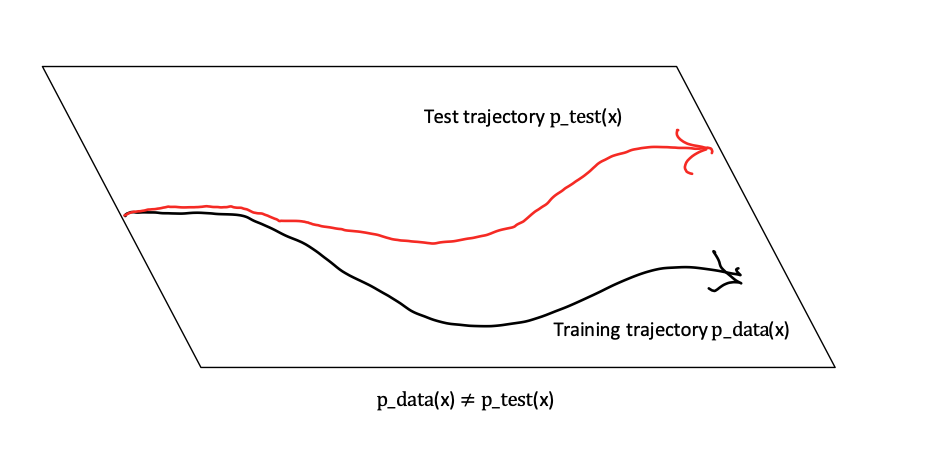
\includegraphics[width=\linewidth]{fig/dilemma.png}
			\caption{Distribution shift illustration}
		  \end{subfigure}%
		  \begin{subfigure}{0.5\linewidth} % Adjust the width as needed
			\centering
			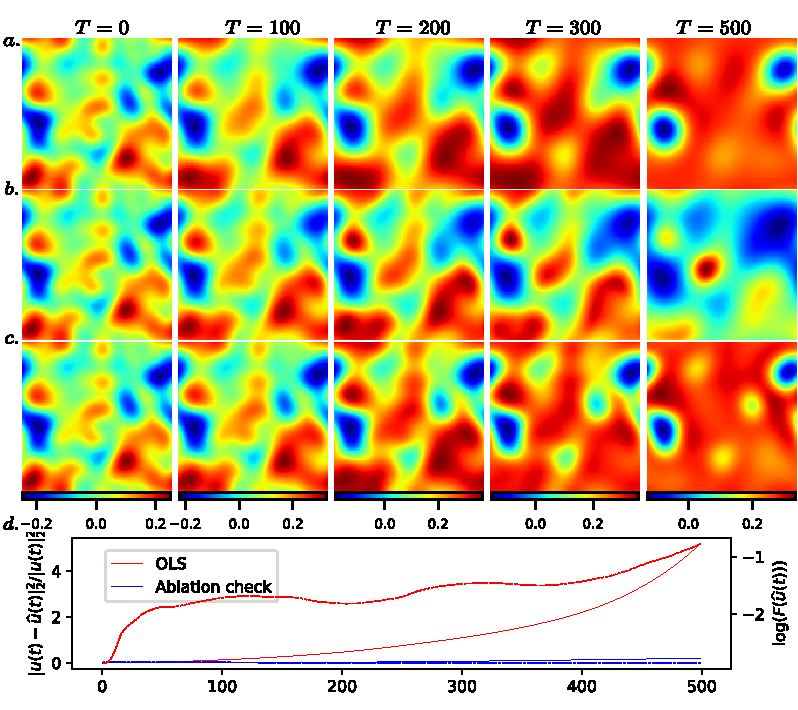
\includegraphics[width=\linewidth]{fig/RD-ds.pdf}
			\caption{Distribution shift in reaction-diffusion equation}
		  \end{subfigure}
	\end{figure}
\end{frame}

\begin{frame}{An heuristic solution}
	\begin{figure}[H]
		\centering
		\centerline{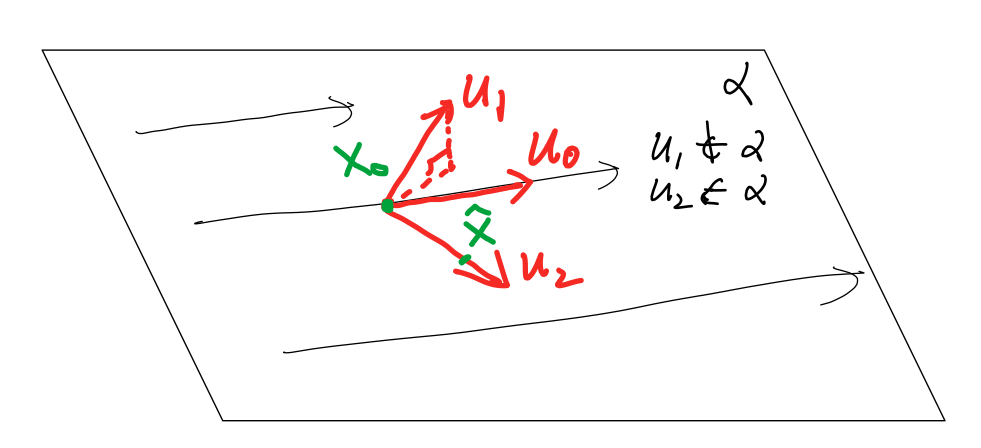
\includegraphics[width=0.9\linewidth]{fig/mfd.png}}
	  \end{figure}
	  We design an algorithm that favours $\mfu_2$ than $\mfu_1$ by adding some regularization.
\end{frame}

\begin{frame}{Network architecture}
	We choose U-net for 
	\begin{figure}[H]
          \centering
          \centerline{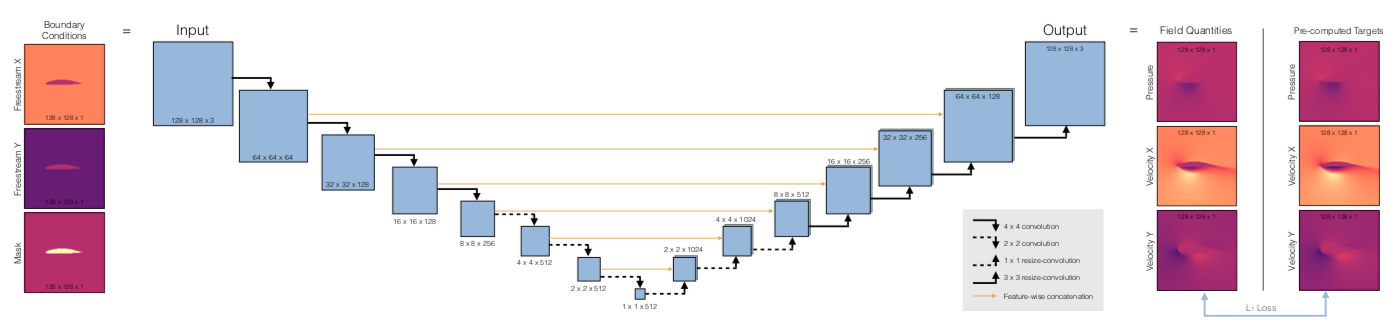
\includegraphics[width=1.1\linewidth]{fig/Unet.png}}
          \caption{U-net structure for flow prediction\footnotemark}
\end{figure}
\footnotetext{Thuerey, Nils, et al. "Deep learning methods for Reynolds-averaged Navier–Stokes simulations of airfoil flows." AIAA Journal 58.1 (2020): 25-36.}
\end{frame}

\begin{frame}{Performance comparison}
	\begin{figure}[H]
          \centering
          \centerline{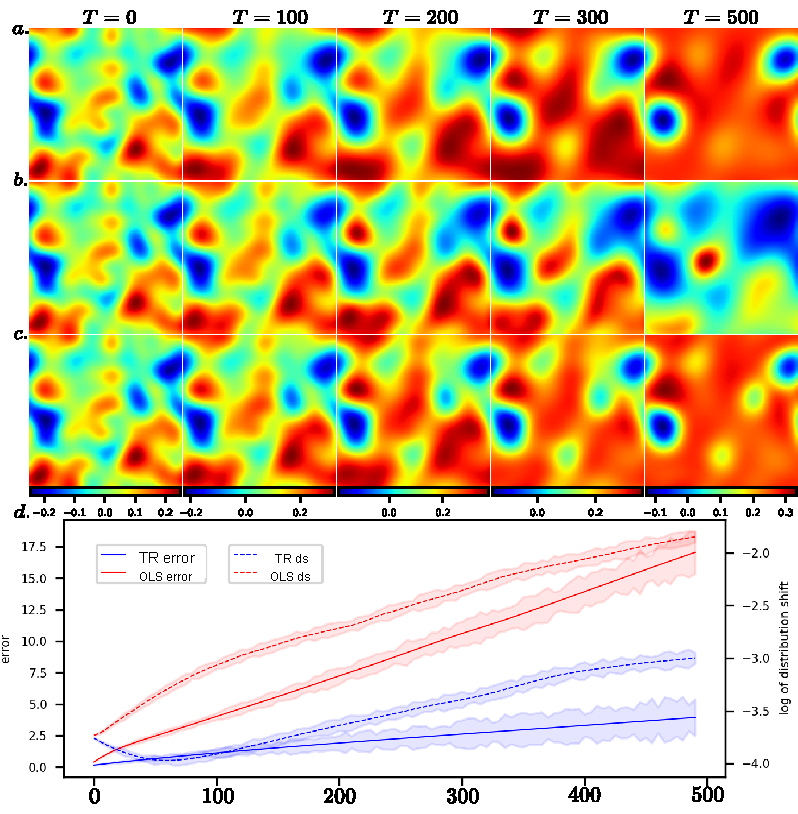
\includegraphics[width=.7\linewidth]{fig/RD-TR.pdf}}
          \caption{Comparison of our method and naive method}
\end{figure}
\end{frame}

\begin{frame}{Performance comparison}
	\begin{figure}[H]
          \centering
          \centerline{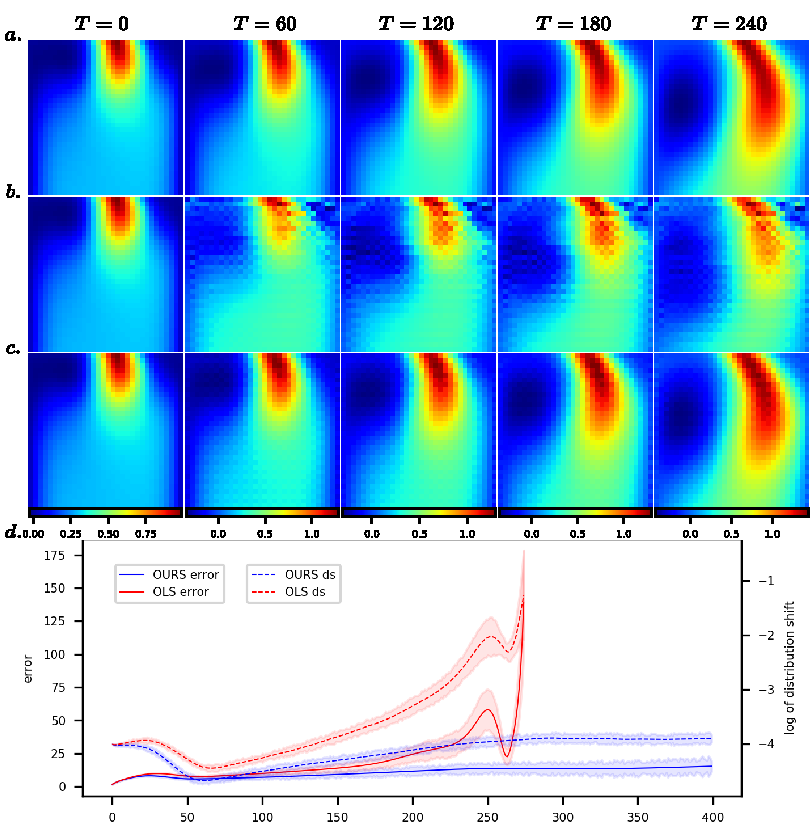
\includegraphics[width=.7\linewidth]{fig/NS-TR.pdf}}
          \caption{Comparison of our method and naive method}
\end{figure}
\end{frame}

\begin{frame}{Further Application}
	\begin{itemize}
		\item 1. Various turbulence modeling: Subgrid modeling, Wall modeling, Transition modeling, etc.
		\item 2. Coupled CFD: Fluid-structure interaction (multiphase flow), flow with heat transfer, etc.
	\end{itemize}
	Iterative solver and data-driven are also presented in these applcations.
\end{frame}

\begin{frame}{The idea of shadowing}
	Consider a parametric dynamics
	\begin{equation}
		\p_t u = f(u, s).
	\end{equation}
	\begin{figure}[H]
          \centering
          \centerline{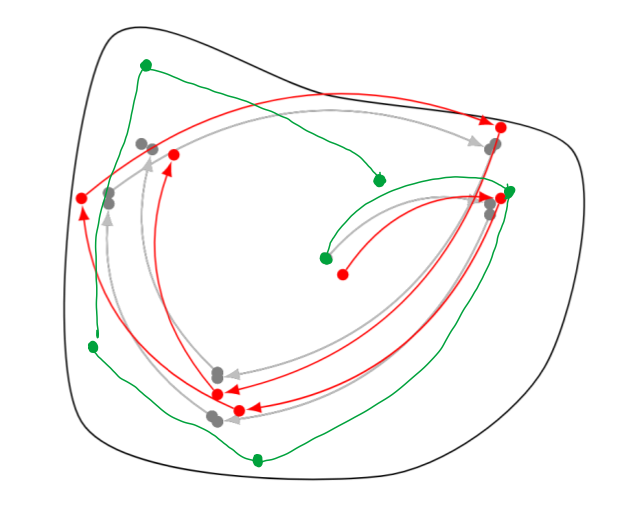
\includegraphics[width=.6\linewidth]{fig/shadowing.png}}
          \caption{Shadowing trajectory: {\color{green} perturbed $s+\delta s$-trajectory} and {\color{red} shadowing $s+\delta s$-trajectory}}
\end{figure}
\end{frame}

\begin{frame}{Solve LSS: Least square}
	Writing the linearized equation as a linear constraint
	\begin{equation}\label{equ:lss}
		\begin{aligned}
			& \min \sum_{t=1}^T v_t^T v_t \\
		&\begin{pmatrix}
			\mfI & -\nabla_u f(u_{T-1}) & \cdots & 0 & 0 \\
			0 & \mfI & \cdots & 0 & 0 \\
			0 & 0 & \cdots & 0 & 0 \\
			\vdots & \vdots & \ddots & \vdots & \vdots \\
			0 & 0 & \cdots & \mfI & -\nabla_u f(u_1)	\\
			0 & 0 & \cdots & 0 & 0
		\end{pmatrix}\begin{pmatrix}
			v_T \\ v_{T-1} \\ v_{T-2} \\ \vdots \\ v_2 \\ v_1
		\end{pmatrix} = \begin{pmatrix}
			\p_s f(u_{T-1}) \\ \p_s f(u_{T-2}) \\ \p_s f(u_{T-3}) \\ \vdots \\ \p_s f(u_{1}) \\ 0
		\end{pmatrix},
	\end{aligned}
	\end{equation}
	This is just a least square problem of size $T \times N$. The huge linear system is the linearized equation.
\end{frame}

\begin{frame}{Sensitivity analysis of the Lorenz system}
	Let us start with the simple 3D Lorenz system (a reduced-order model for heat transfer flow) with a parameter $\rho$ (Reyleigh number)
	\begin{equation}
		J(\rho) := \lim_{T\rightarrow \infty} \frac{1}{T}\int_0^T z_{\rho}(t)dt.
	\end{equation} 
	\begin{figure}[ht]
			\centering
			\begin{subfigure}{0.5\linewidth} % Adjust the width as needed
				\centering
				\includegraphics[width=\linewidth]{fig/Lorenz1.pdf}
				\caption{Gradient calcuated using naive method}
			  \end{subfigure}%
			  \begin{subfigure}{0.5\linewidth} % Adjust the width as needed
				\centering
				\includegraphics[width=\linewidth]{fig/Lorenz2.pdf}
				\caption{Gradient calcuated using LSS}
			  \end{subfigure}
			  \caption{Comparison of naive and LSS methods for sensitivity analysis}
	\end{figure}
\end{frame}

\begin{frame}{Inverse problem for KS equation}
	Consider the 1D Kuramoto–Sivashinsky equation:
	\bequ\label{KS}
		\p_t u + uu_x + u_{xx} + \nu u_{xxxx} = 0, \quad x \in [0, L],
	\eequ
	\begin{figure}[ht]
		\centering
		\begin{subfigure}{0.5\linewidth} % Adjust the width as needed
			\centering
			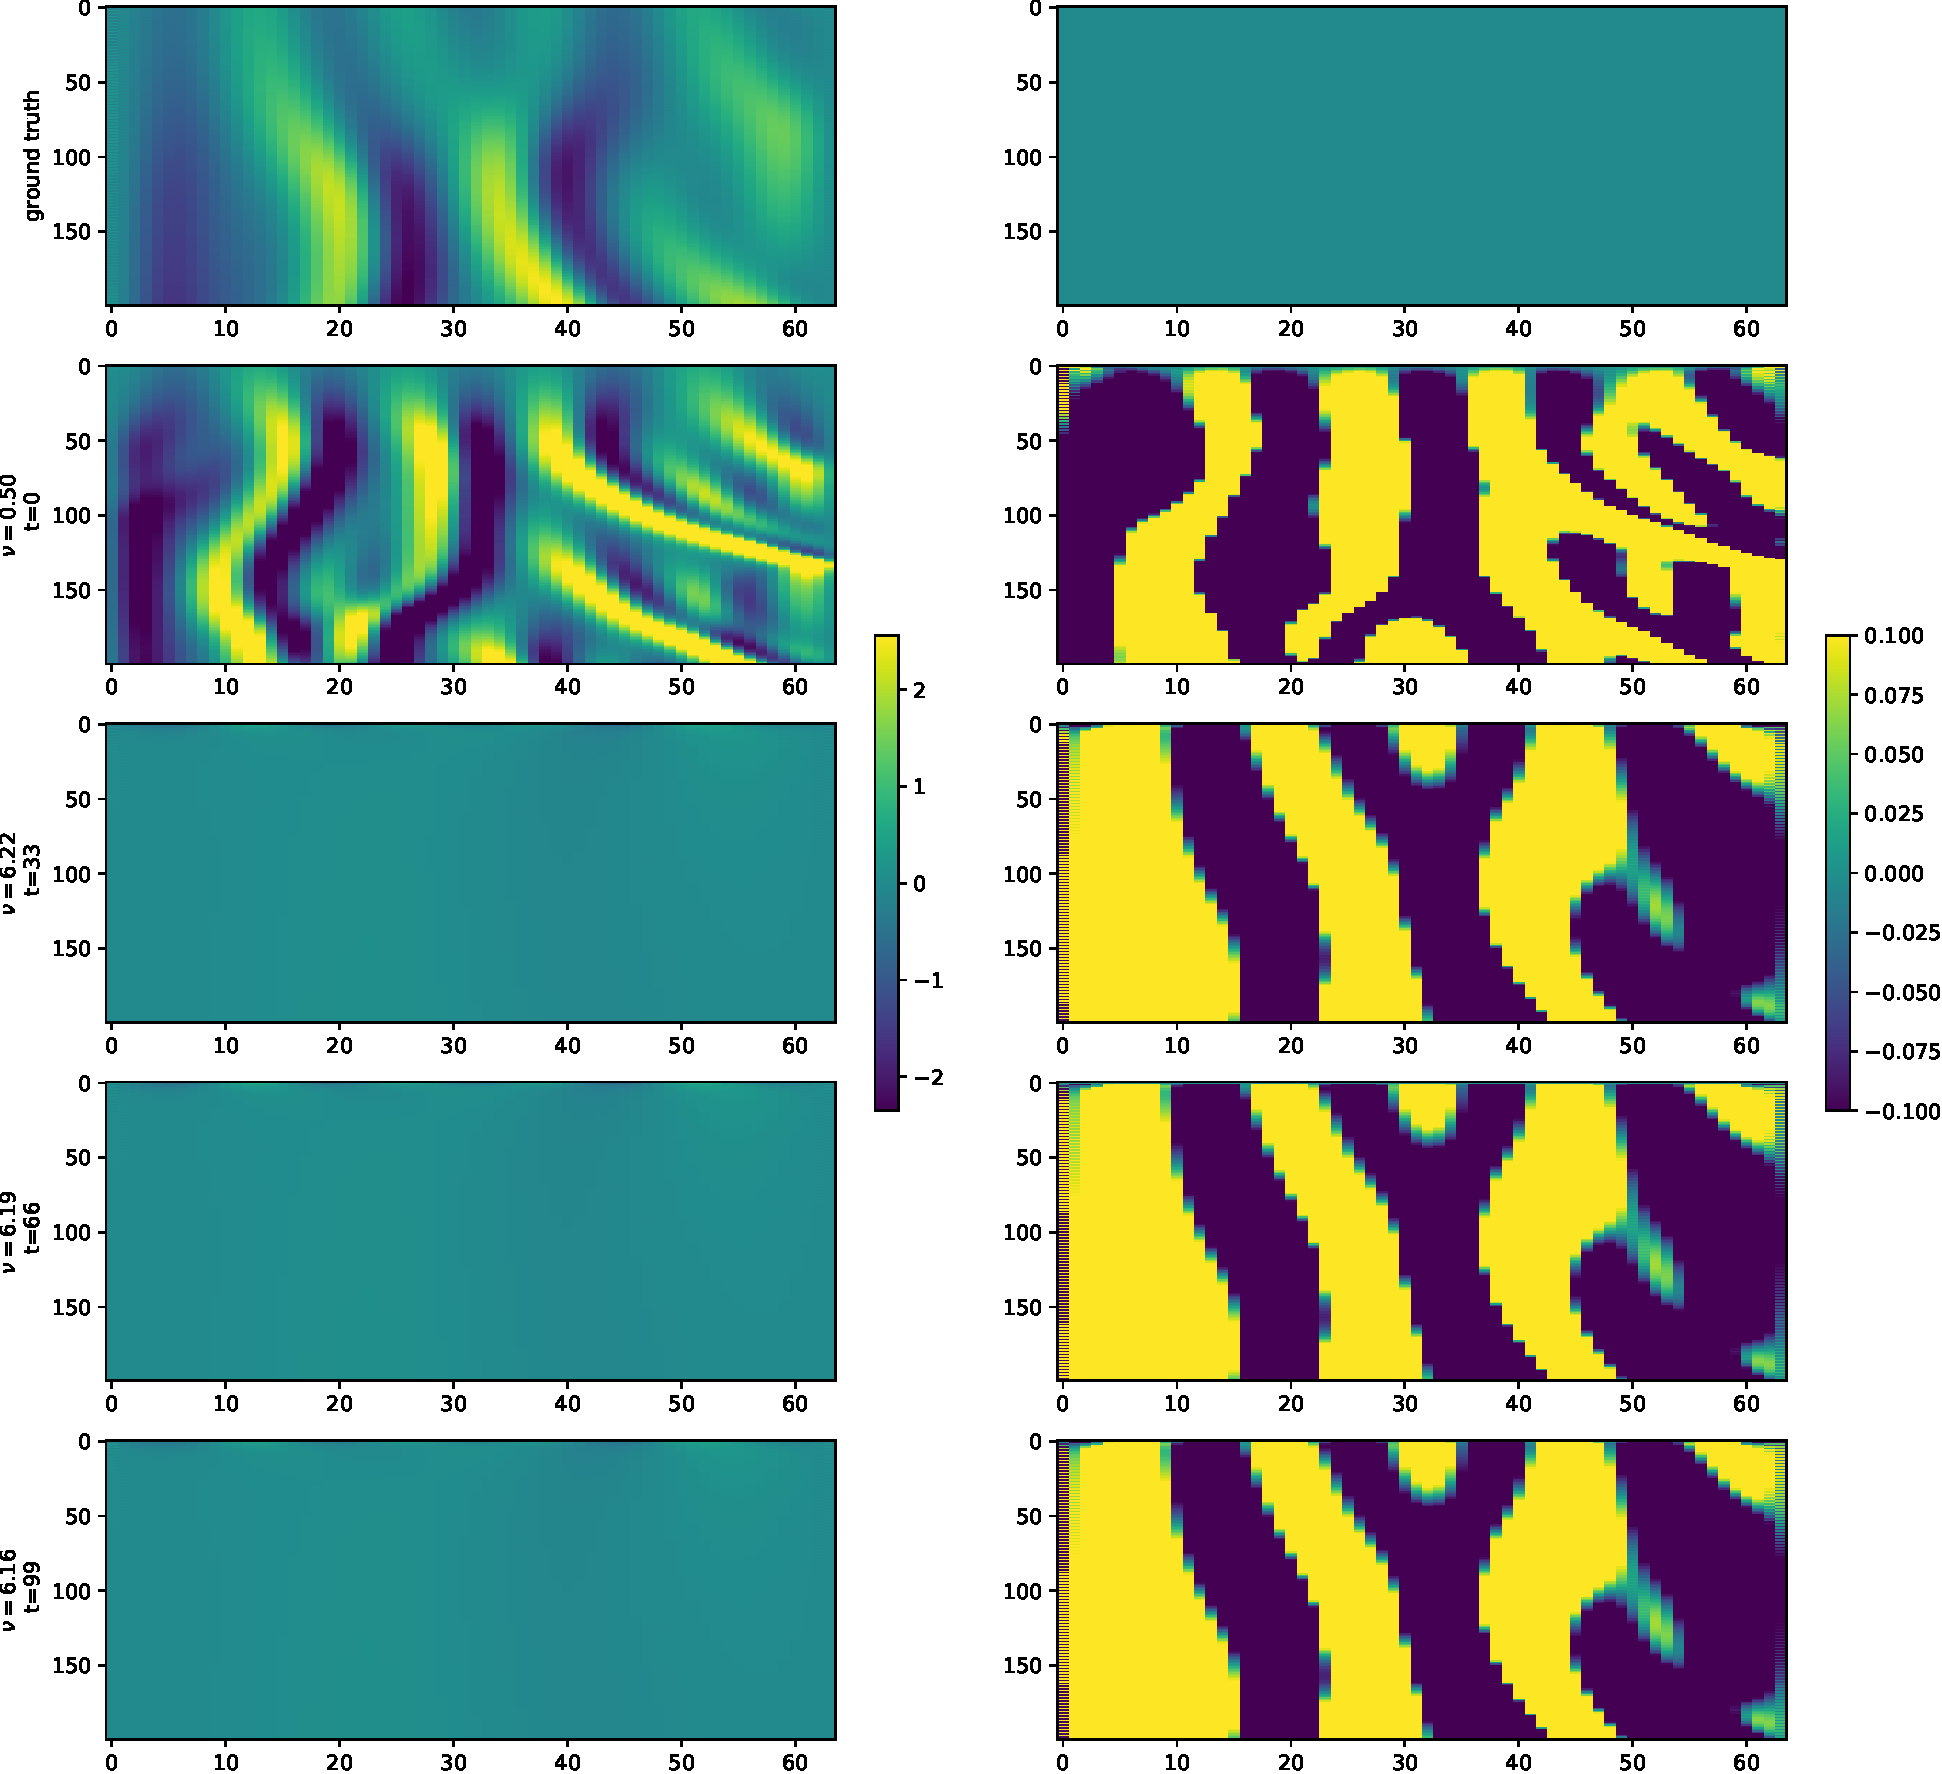
\includegraphics[width=\linewidth]{fig/ks-adjoint-cloudmap2.pdf}
			\caption{Optimization using adjoint method}
		  \end{subfigure}%
		  \begin{subfigure}{0.5\linewidth} % Adjust the width as needed
			\centering
			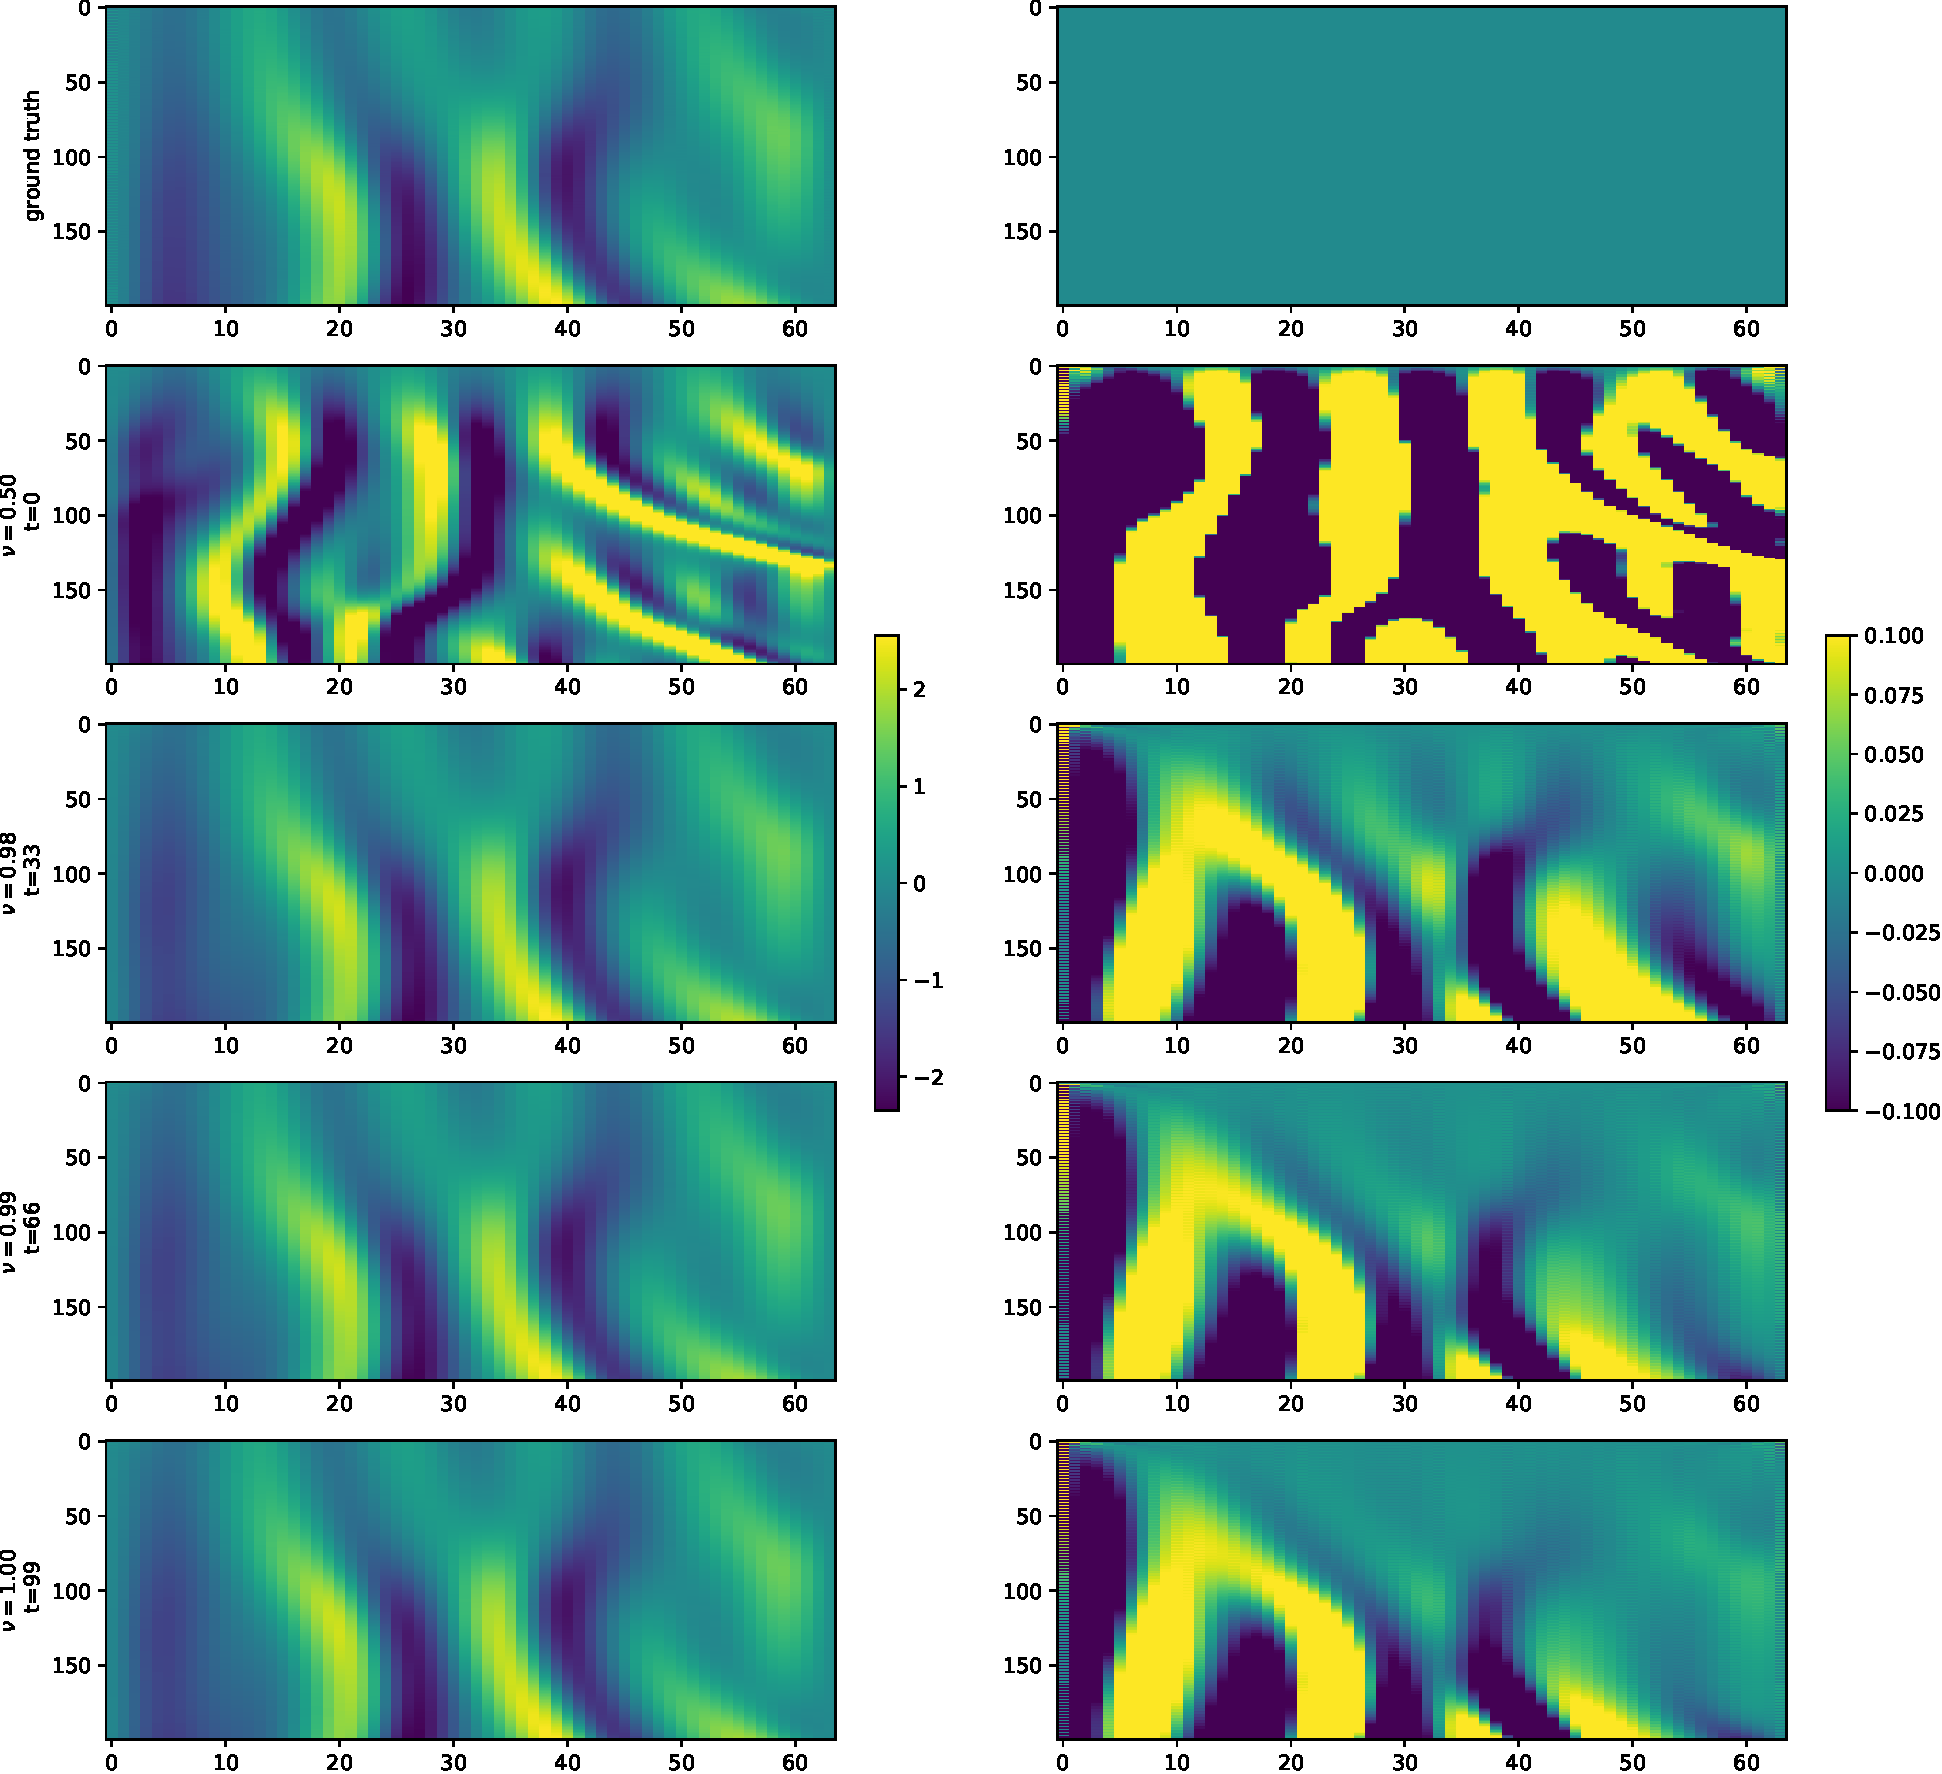
\includegraphics[width=\linewidth]{fig/ks-lss-cloudmap.pdf}
			\caption{Optimization using LSS}
		  \end{subfigure}
		  \caption{Performance of LSS}
	\end{figure}
\end{frame}

\begin{frame}{Sensitivity analysis of LES subgrid modeling}
	\textbf{Difficulties: } We need to solve a linear system of size $N \times T$, with $N$ the number of cells or grid points and $T$ the 
	number of time steps. This is computationally prohibited for even moderate LES.
	\begin{figure}[H]
		\centering
		\centerline{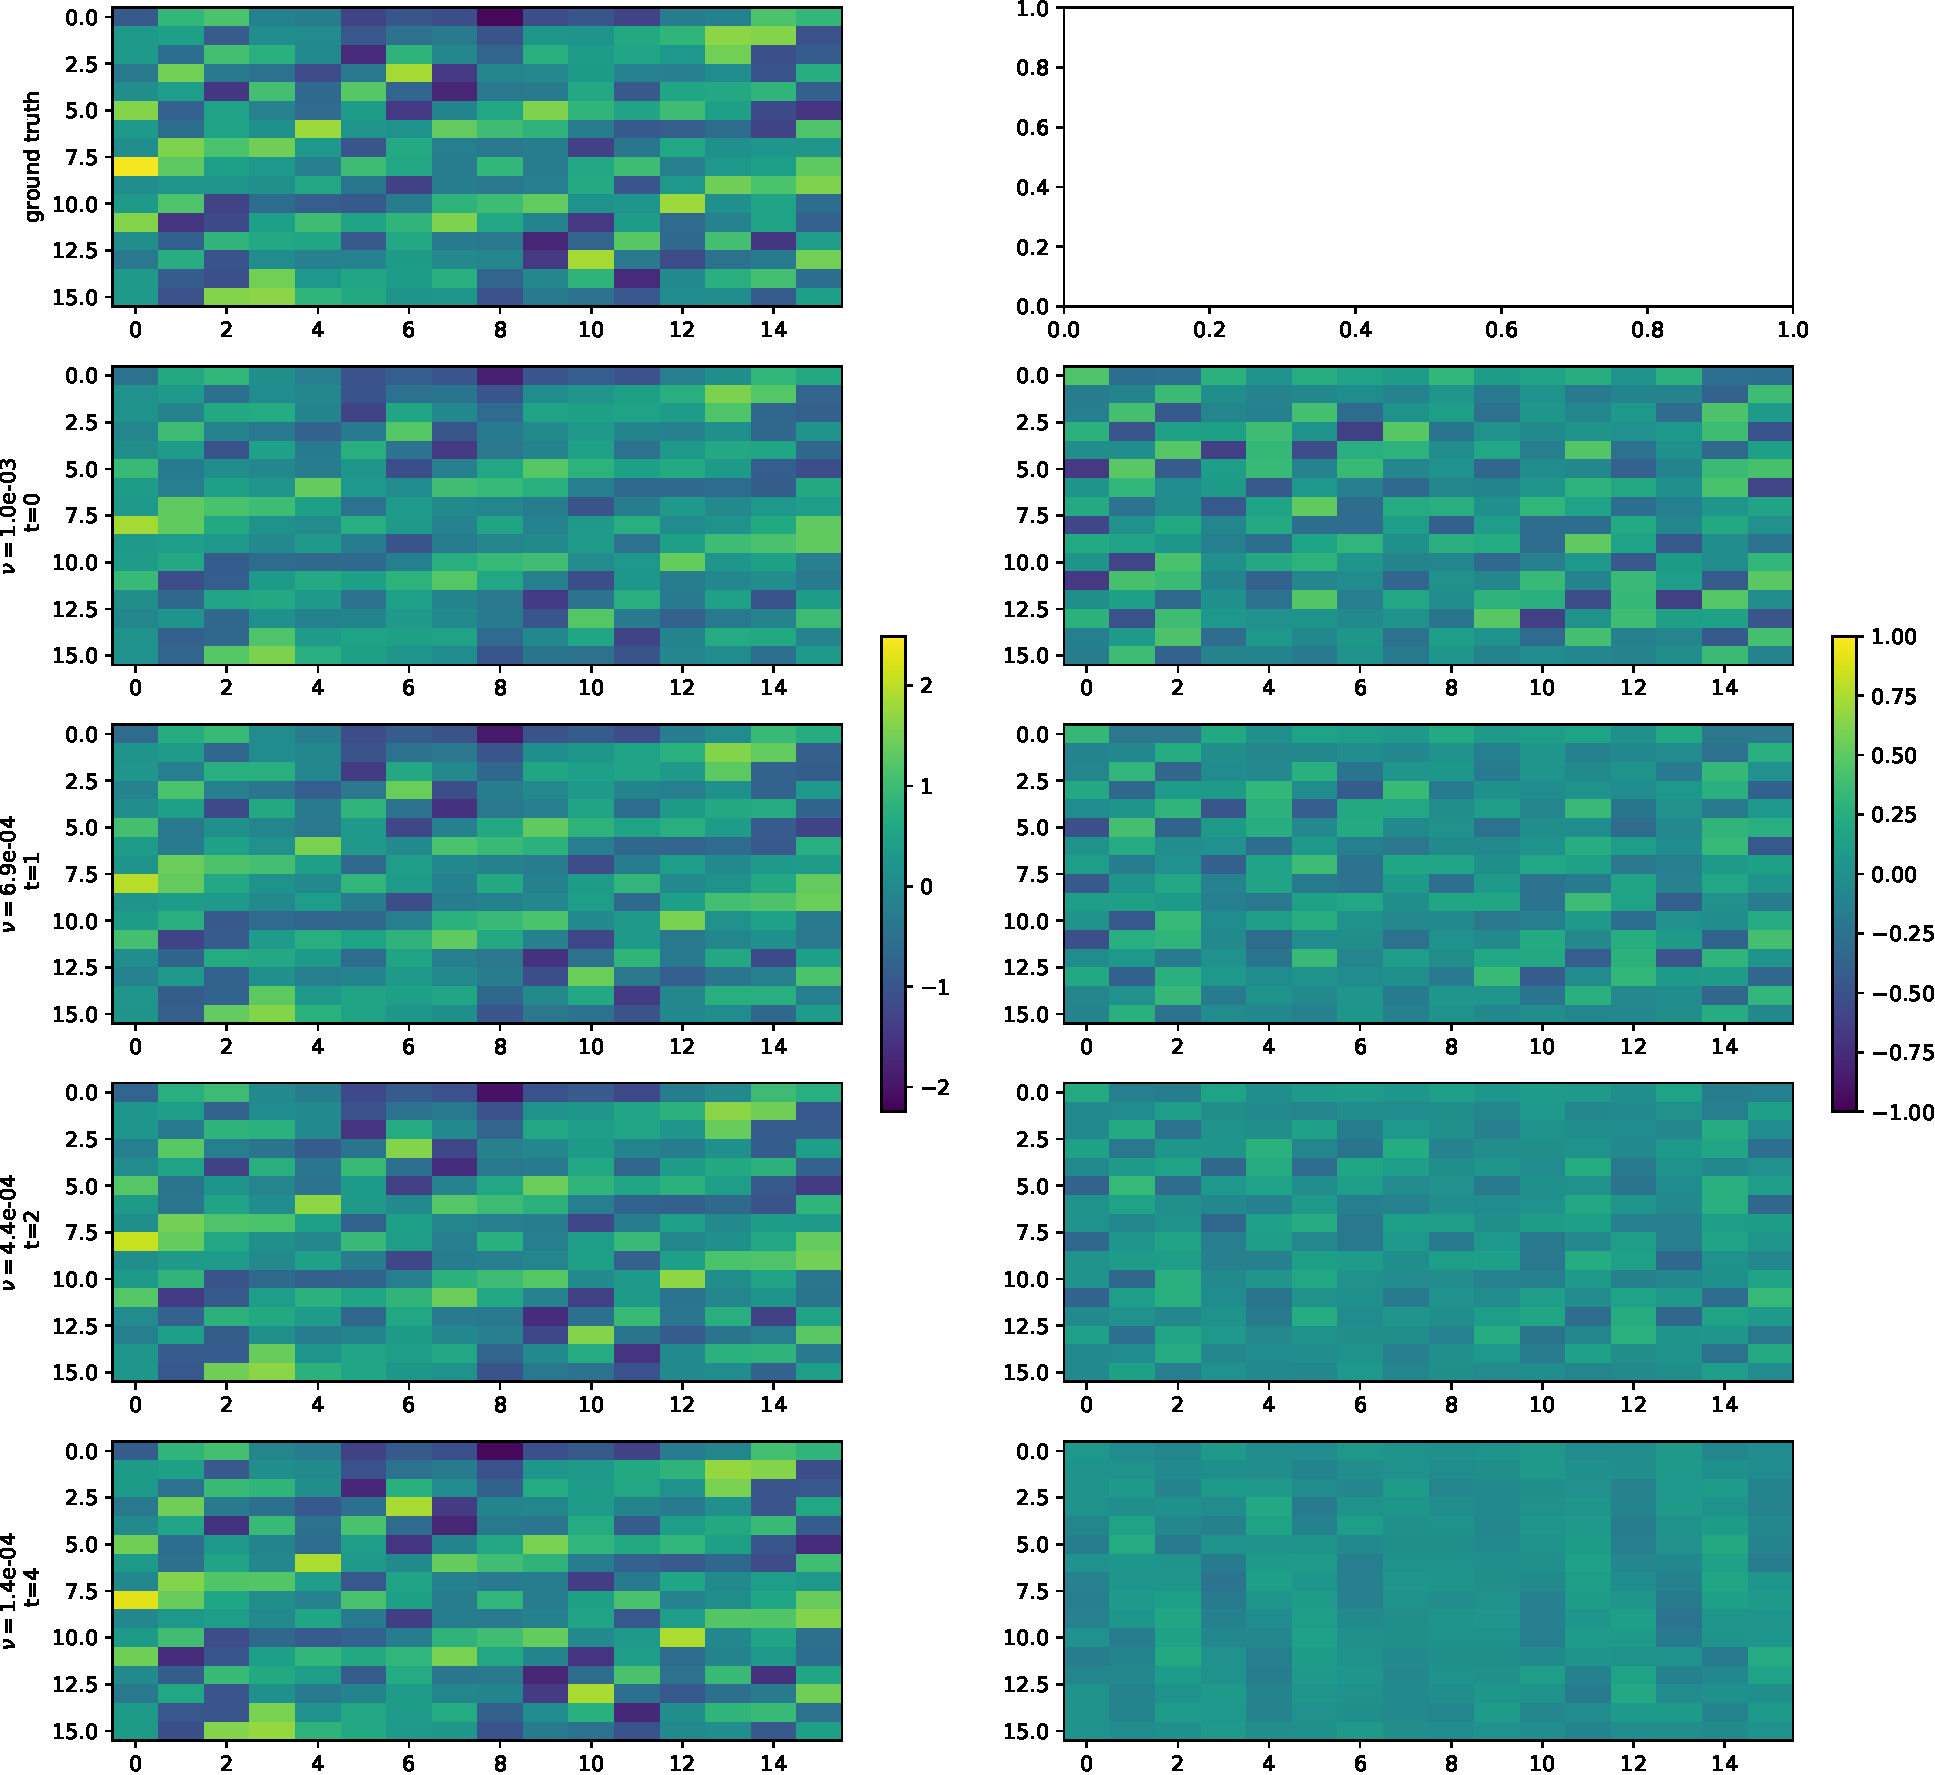
\includegraphics[width=.55\linewidth]{fig/ns-lss-cloudmap.pdf}}
		\caption{Subgrid modeling of NS equation in 2D}
\end{figure}
\end{frame}

\begin{frame}{Sensitivity analysis of LES subgrid modeling}
	\textbf{Then, why not have a try with machine learning?}
	\begin{equation}
		\mfu \overset{NN}{\Longrightarrow} v_1.
	\end{equation}
	\begin{itemize}
		\item 1. Seq2Seq processing
		\item 2. Using the idea of Neural radiance field (NeRF) to directly learn the policy
		\item 3. Unsupervised learning or Reinforcement learning
	\end{itemize}
\end{frame}

\begin{frame}{Application}
	\begin{itemize}
		\item 1. Flow control
		\item 2. Inverse design \& shape optimization
		\item 3. Uncertainty quantification of fluid system
	\end{itemize}
\end{frame}

\begin{frame}{Appendix: Reaction-diffusion equation}
	Consider following FitzHugh-Nagumo reaction diffusion equation:
	\begin{equation}
    \begin{aligned}
        	\frac{\p \mfu}{\p t} & = \gamma \Delta \mfu + \mfR(\mfu), \quad T \in [0, 1], 	\\
		\mfR(\mfu) & = \mfR(u, v) = \begin{pmatrix}
			u - u^3 - v - \alpha	\\
			\beta(u - v)
		\end{pmatrix},
    \end{aligned}
	\end{equation}
	The initial data is given by $\mfu_0$ is a random field and generated by i.i.d. sampling from a normal distribution and $\alpha = 0.001, \beta=1.0, \gamma = \begin{pmatrix}
		0.05 & 0	\\
		0 & 0.1
	\end{pmatrix}$. We use mesh size $128 \times 128$ for the whole problems. Computational domain is given by $[0, 6.4]\times[0, 6.4]$.
\end{frame}

\begin{frame}{Appendix: Shadowing lemma}
	\begin{theorem}[Shadowing lemma]
		Let $\Gamma$ be a hyperbolic invariant set of a diffeomorphism $f$. There exists a 
		neighborhood $U$ of $\Gamma$ with the following property: for any $\delta > 0$ there 
		exists $\epsilon > 0$, such that any (finite or infinite) $\epsilon$-pseudo-orbit that 
		stays in $U$ also stays in a $\delta$-neighborhood of some true orbit\footnotemark.
	\end{theorem}
	In a hyperbolic invariant set, the dynamics exhibit a combination of stable and unstable behavior.

	\href{https://www.youtube.com/watch?v=07jkQ1ox7vI&t=290s}{\textbf{Shadowing trajectory demo:}}
	\footnotetext{Pilyugin SY. Shadowing in dynamical systems. Lecture notes in mathematics, vol. 1706. Springer; 1999.}
\end{frame}
\end{document}